\documentclass[12pt,a4paper]{article}
\usepackage[utf8]{inputenc}
\usepackage[russian]{babel}
\usepackage{amsmath, amssymb, amsfonts}
\usepackage{graphicx}
\usepackage{float}
\usepackage{geometry}
\geometry{left=2.5cm, right=2cm, top=2cm, bottom=2cm}
\usepackage{indentfirst}
\usepackage{caption}
\usepackage{xcolor}

\begin{document}


\title{\begin{center}Лабораторная работа № 5.5.5\end{center}
Компьютерная сцинтилляционная $\gamma$-спектрометрия}
\author{Струков О. И. \\ Б04-404}
\date{}

\thispagestyle{empty}
\pagenumbering{gobble}
\maketitle
\newpage
\pagenumbering{arabic}

\section*{Теоретическая часть}

\subsection*{1. Взаимодействие $\gamma$-излучения с веществом}
При прохождении гамма-квантов через материальную среду основными процессами их взаимодействия с веществом являются:
\begin{enumerate}
    \item \textbf{Фотоэффект} --- процесс, при котором $\gamma$-квант полностью поглощается атомом, передавая всю свою энергию $E_\gamma$ одному из связанных электронов. Кинетическая энергия выбитого электрона равна $T_e = E_\gamma - I_i$, где $I_i$ --- потенциал ионизации оболочки. Вероятность фотоэффекта резко возрастает с увеличением атомного номера вещества ($\propto Z^5$) и падает с ростом энергии кванта.
    \item \textbf{Эффект Комптона} --- упругое рассеяние фотона на слабосвязанных (практически свободных) электронах атомной оболочки, сопровождающееся изменением длины волны фотона. При этом электрону передаётся лишь часть энергии $\gamma$-кванта.
    \item \textbf{Рождение электрон-позитронных пар} --- пороговый процесс, возможный в кулоновском поле ядра при энергии $\gamma$-кванта $E_\gamma \geqslant 2mc^2 \approx 1,022$ МэВ. Избыток энергии переходит в кинетическую энергию образовавшихся частиц.
\end{enumerate}

\subsection*{2. Принцип действия сцинтилляционного детектора}
В данной работе используется сцинтилляционный спектрометр на основе монокристалла йодида натрия, активированного таллием --- NaI(Tl). 

При взаимодействии $\gamma$-кванта с кристаллом образуются быстрые электроны, которые возбуждают атомы решётки. При релаксации возникает световая вспышка. Чистый кристалл NaI сильно поглощает собственное излучение, поэтому в него вводят примесь таллия (около 0,1\%). Уровни энергии таллия находятся в запрещённой зоне кристалла, и излучаемые при переходах на них фотоны имеют меньшую энергию, не поглощаются решёткой и свободно выходят из кристалла.

Световая вспышка попадает на фотокатод фотоэлектронного умножителя (ФЭУ), где за счёт внешнего фотоэффекта выбиваются электроны. Они ускоряются и умножаются в системе динодов ФЭУ. В результате на аноде формируется электрический импульс, амплитуда которого строго пропорциональна энергии, потерянной $\gamma$-квантом в кристалле.

\subsection*{3. Структура гамма-спектра}
Спектр, регистрируемый амплитудным анализатором, имеет характерную форму (рис. 1), обусловленную разными механизмами взаимодействия:

% === МЕСТО ДЛЯ ВСТАВКИ СХЕМЫ СПЕКТРА ===
\begin{figure}[htbp]
    \centering
    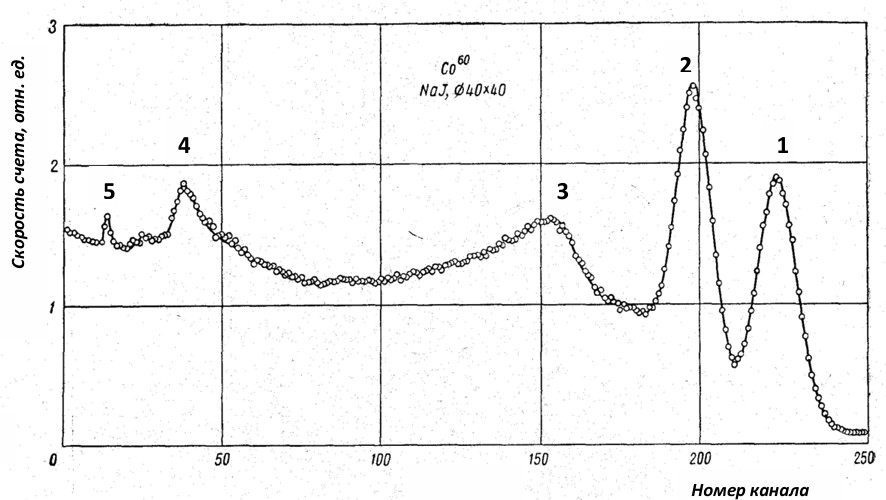
\includegraphics[width=0.6\textwidth]{1.jpg}
    % \fbox{\parbox{0.8\textwidth}{\centering\vspace{2.5cm} \textit{Вставьте сюда Рис. из методички: Типичный спектр $^{137}$Cs или $^{60}$Co с подписанными фотопиком, комптоновским краем и пиком обратного рассеяния} \vspace{2.5cm}}}
    \caption{Типичный спектр $\gamma$-излучения $^{60}Co$ (1 и 2 -- фотопики, 3 -- край комптоновского спектра, 4 -- пик обратного рассеяния, 5 -- пик характеристического излучения свинца)}
    \label{fig:spectrum}
\end{figure}

\begin{itemize}
    \item \textbf{Фотопик (пик полного поглощения)} --- возникает, когда $\gamma$-квант передаёт кристаллу всю свою энергию $E_\gamma$ (обычно в результате фотоэффекта или многократного комптоновского рассеяния с последующим фотоэффектом).
    \item \textbf{Комптоновское плато и край} --- непрерывное распределение, обусловленное комптоновским рассеянием внутри кристалла, когда рассеянный фотон покидает его. Максимальная энергия, передаваемая электрону (комптоновский край), соответствует рассеянию на угол $180^\circ$:
    \begin{equation}
        E_{\text{max}} = E_\gamma \frac{2E_\gamma}{2E_\gamma + mc^2}.
    \end{equation}
    \item \textbf{Пик обратного рассеяния} --- образуется $\gamma$-квантами, которые испытали комптоновское рассеяние на угол $\approx 180^\circ$ на материалах защиты (например, свинце) и затем попали в детектор. Его энергия определяется формулой:
    \begin{equation}
        E_{\text{обр}} = \frac{E_\gamma}{1 + 2E_\gamma / mc^2}.
    \end{equation}
    \item \textbf{Аннигиляционный пик} --- характерен для $\beta^+$-источников (например, $^{22}$Na). Позитроны аннигилируют в веществе, рождая два $\gamma$-кванта по $511$ кэВ каждый.
\end{itemize}

\subsection*{4. Энергетическое разрешение спектрометра}
Даже для моноэнергетических $\gamma$-квантов фотопик имеет конечную ширину, описываемую гауссовым распределением. Это связано со статистическим характером процессов преобразования энергии (рождение фотонов, сбор света на фотокатоде, умножение в ФЭУ). 

Число фотоэлектронов $n$, собираемых на первом диноде, подчиняется распределению Пуассона, поэтому его среднеквадратичная флуктуация равна $\Delta n = \sqrt{n}$. Поскольку энергия $E \propto n$, а ширина пика на полувысоте $\Delta E \propto \Delta n$, статистический вклад в энергетическое разрешение $R$ имеет вид:
\begin{equation}
    R = \frac{\Delta E}{E} \cdot 100\% \propto \frac{1}{\sqrt{E}}.
\end{equation}
На практике разрешение ухудшается из-за неоднородности светосбора в кристалле и электронных шумов, поэтому зависимость от энергии остаётся обратной, но с большим коэффициентом.

\subsection*{5. Калибровка спектрометра}
Для перевода номеров каналов амплитудного анализатора $N$ в энергетические единицы (МэВ) используется линейная калибровочная зависимость, справедливая для ФЭУ в рабочем диапазоне:
\begin{equation}
    N_i = a E_i + b,
\end{equation}
где $E_i$ --- табличные энергии $\gamma$-линий известных источников (например, $^{60}$Co с линиями $1,17$ МэВ и $1,33$ МэВ, или $^{137}$Cs с линией $0,662$ МэВ), а $a$ и $b$ --- коэффициенты, определяемые методом наименьших квадратов.


\section*{Ход работы}

\subsection*{1. Калибровка гамма-спектрометра}

Для перевода номеров каналов амплитудного анализатора в энергетические единицы (МэВ) была проведена калибровка спектрометра по известным энергиям $\gamma$-линий радиоактивных источников. Зависимость номера канала от энергии аппроксимировалась линейной функцией:
\begin{equation}
    N_i = a E_i + b,
\end{equation}
где $N_i$ --- номер канала, соответствующий центру фотопика, $E_i$ --- табличная энергия $\gamma$-кванта, $a$ и $b$ --- калибровочные коэффициенты.

Для калибровки использовались фотопики следующих источников:
\begin{itemize}
    \item $^{22}$Na: аннигиляционный пик ($0,511$ МэВ) и фотопик ($1,274$ МэВ);
    \item $^{137}$Cs: фотопик ($0,662$ МэВ);
    \item $^{60}$Co: два фотопика ($1,173$ МэВ и $1,333$ МэВ).
\end{itemize}

Результаты измерений положений фотопиков представлены в таблице 1.

\begin{table}[H]
\centering
\caption{Данные для калибровки гамма-спектрометра}
\label{tab:calibration}
\renewcommand{\arraystretch}{1.2}
\begin{tabular}{|c|c|c|}
\hline
Источник & $N_i$ & $E_i$, МэВ \\
\hline
$^{22}$Na & $747,769 \pm 58,799$ & $0,511$ \\
$^{137}$Cs & $950,315 \pm 63,549$ & $0,662$ \\
$^{60}$Co & $1637,490 \pm 85,430$ & $1,173$ \\
$^{22}$Na & $1761,878 \pm 108,979$ & $1,274$ \\
$^{60}$Co & $1849,134 \pm 93,856$ & $1,333$ \\
\hline
\end{tabular}
\end{table}

По данным таблицы был построен калибровочный график и проведена линейная аппроксимация методом наименьших квадратов (рис. 1).

\begin{figure}[H]
    \centering
    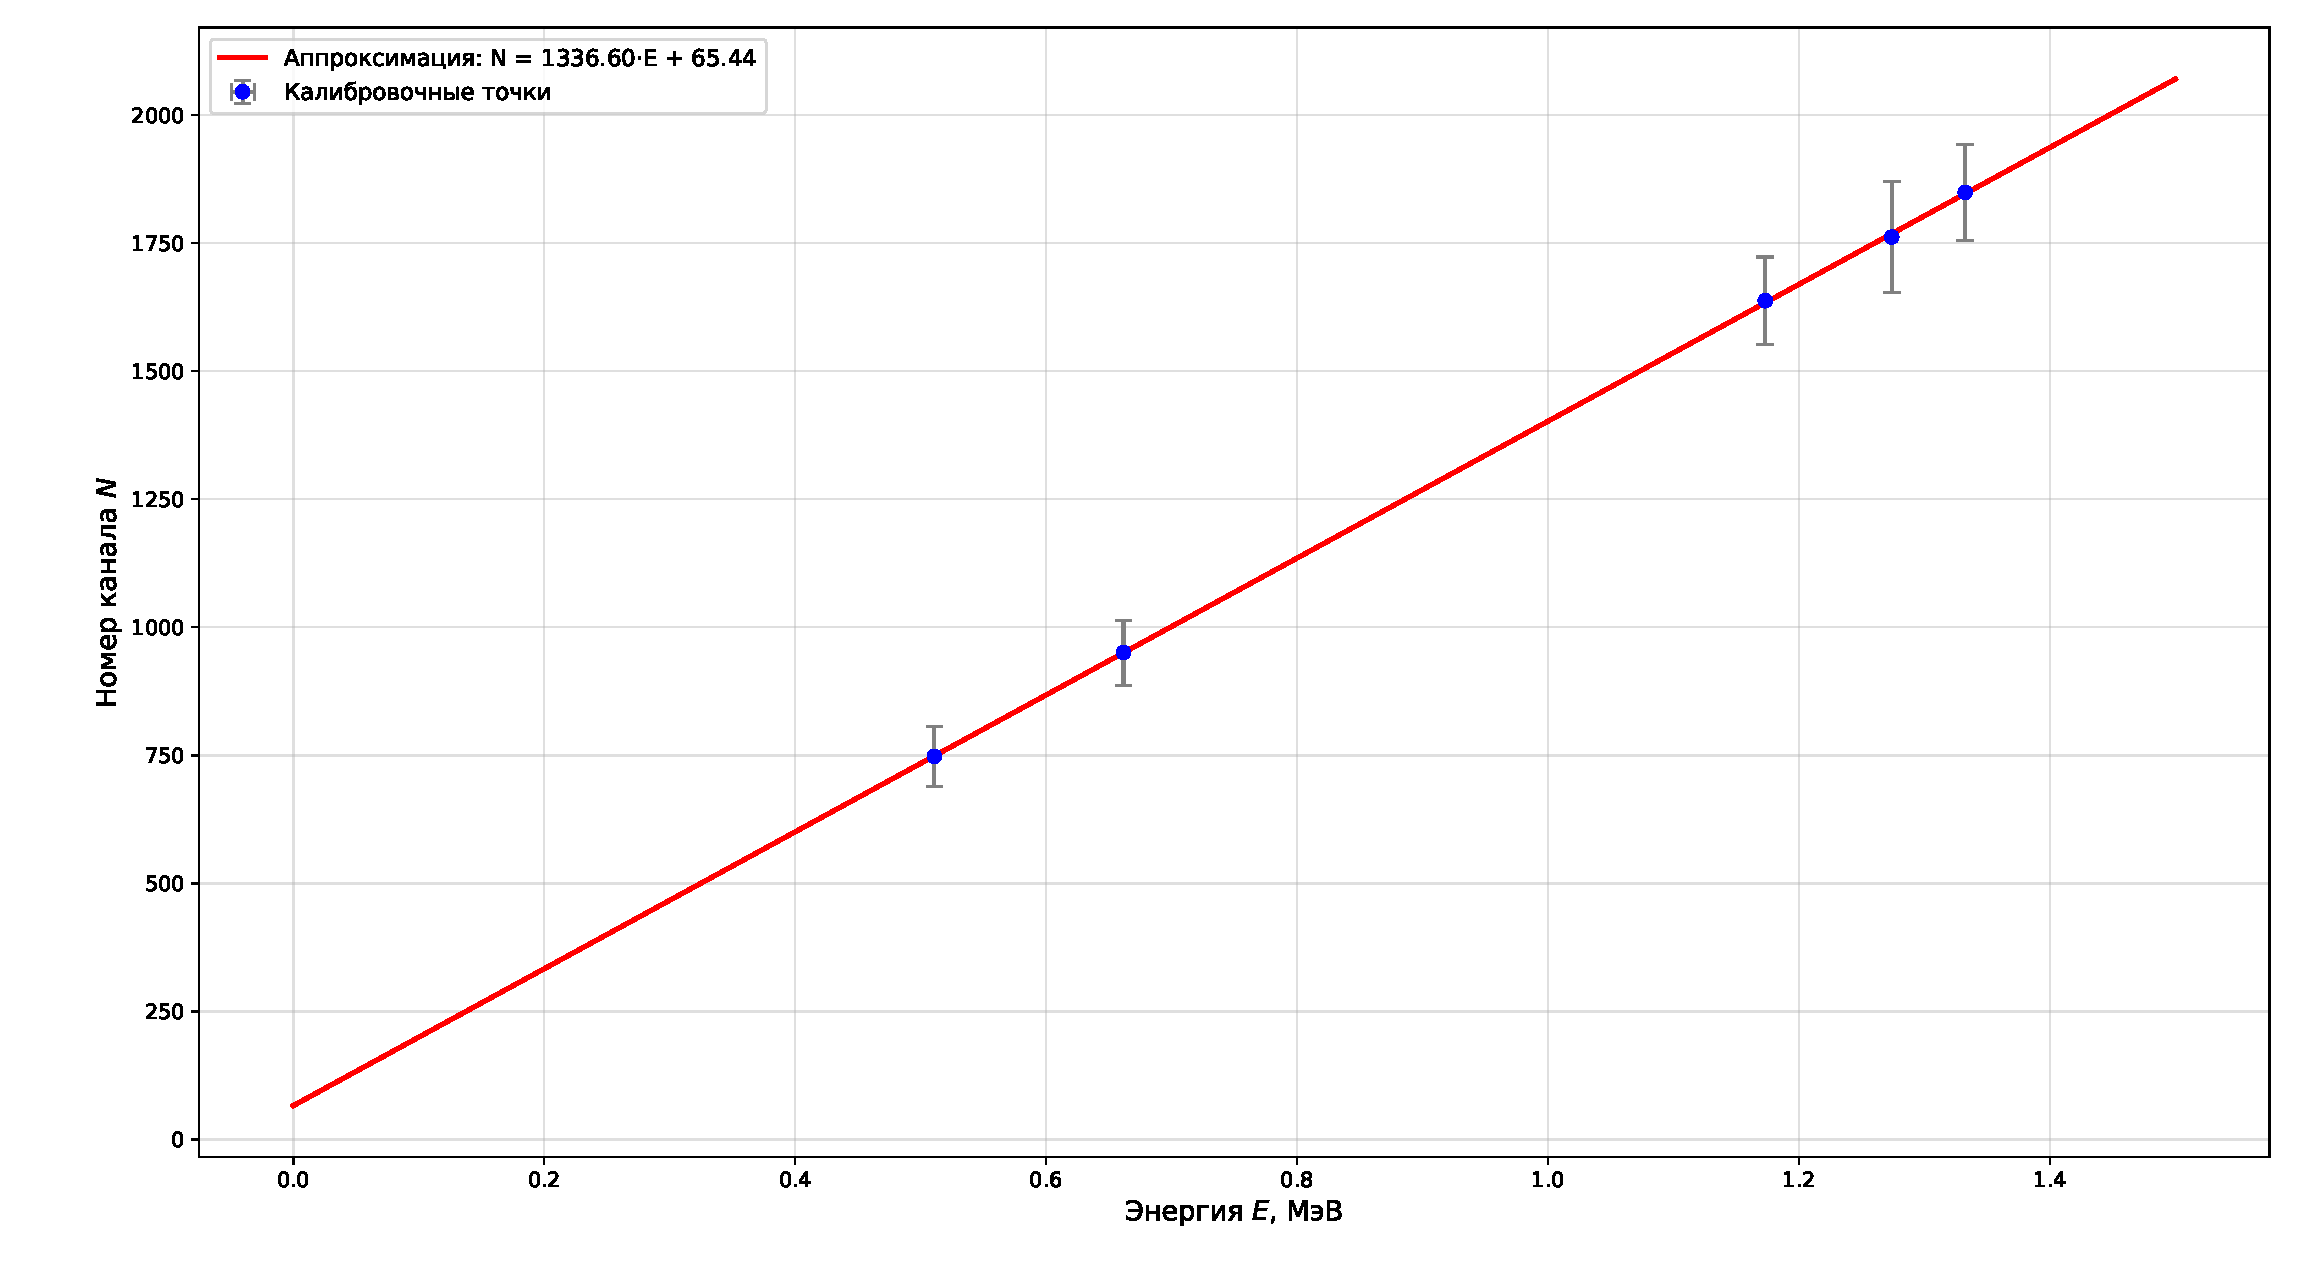
\includegraphics[width=0.8\textwidth]{2.pdf}
    \caption{Калибровочный график зависимости номера канала от энергии $\gamma$-кванта.}
    \label{fig:calibration}
\end{figure}

В результате аппроксимации методом наименьших квадратов были получены следующие значения коэффициентов:
\begin{equation}
    a = (1336,60 \pm 6,14) \text{ каналов/МэВ}, \quad b = (65,44 \pm 6,42) \text{ каналов}.
\end{equation}% \textit{(Здесь подставьте точные значения $a$ и $b$, которые выдаст Python-скрипт!)}

% Коэффициент детерминации $R^2 \approx 0,999$, что подтверждает высокую линейность отклика спектрометра в исследуемом диапазоне энергий. 
В дальнейшем для определения энергии неизвестных пиков будет использоваться формула:
\begin{equation}
    E_i = \frac{N_i - b}{a}.
\end{equation}


\subsection*{1. Обработка результатов и калибровка}

Для перевода номеров каналов в энергетические единицы была использована линейная калибровочная зависимость, полученная по фотопикам известных источников:
\begin{equation}
    N = 1336,60 \cdot E + 65,44 \quad \implies \quad E = \frac{N - 65,44}{1336,60},
\end{equation}
где $N$ --- номер канала, $E$ --- энергия в МэВ.

Результаты обработки всех зарегистрированных спектров (включая пики полного поглощения, комптоновские края и фоновые пики) сведены в таблицу 1. Погрешность энергии $\Delta E_i$ рассчитывалась как $\Delta N_i / 1336,60$, а энергетическое разрешение --- как $R_i = \Delta E_i / E_i$.

% В преамбуле добавьте: \usepackage{xcolor}

\begin{table}[H]
\centering
\caption{Результаты обработки гамма-спектров: положения пиков, энергии и разрешение. Табличные значения энергий выделены зелёным цветом.}
\label{tab:gamma_spectra_results}
\renewcommand{\arraystretch}{1.1}
\resizebox{\textwidth}{!}{%
\begin{tabular}{|c|c|c|c|c|c|c|}
\hline
Источник & $N_i$ & $\Delta N_i$ & $E_i$, МэВ & $\Delta E_i$, МэВ & $R_i$ & Тип излучения \\
\hline
$^{60}$Co   & 163,18 & 27,28 & 0,073 & 0,020 & 0,279 & Излучение Pb \\
$^{60}$Co   & 371,01 & 75,62 & 0,229 & 0,057 & 0,248 & Пик обратного рассеяния \\
$^{60}$Co   & 1264,81 & 122,81 & 0,897 & 0,092 & 0,102 & Край компт. спектра \\
$^{60}$Co   & 1637,49 & 85,43 & \textcolor{green!60!black}{\textbf{1,173}} & 0,064 & 0,054 & Фотопик \\
$^{60}$Co   & 1849,13 & 93,86 & \textcolor{green!60!black}{\textbf{1,333}} & 0,070 & 0,053 & Фотопик \\
\hline
$^{137}$Cs  & 98,11 & 12,96 & 0,024 & 0,010 & 0,397 & Излучение Ba \\
$^{137}$Cs  & 164,95 & 20,31 & 0,074 & 0,015 & 0,204 & Излучение Pb \\
$^{137}$Cs  & 329,77 & 89,07 & 0,198 & 0,067 & 0,337 & Пик обратного рассеяния \\
$^{137}$Cs  & $\sim$ 700 & -- & $\sim$ 0,475 & -- & -- & Край компт. спектра \\
$^{137}$Cs  & 950,32 & 63,55 & \textcolor{green!60!black}{\textbf{0,662}} & 0,048 & 0,072 & Фотопик \\
\hline
$^{22}$Na   & 167,22 & 22,10 & 0,076 & 0,017 & 0,217 & Излучение Pb \\
$^{22}$Na   & 302,90 & 125,02 & 0,178 & 0,094 & 0,527 & Пик обратного рассеяния \\
$^{22}$Na   & 437,69 & 113,27 & 0,279 & 0,085 & 0,304 & Край компт. спектра \\
$^{22}$Na   & 747,77 & 58,80 & \textcolor{green!60!black}{\textbf{0,511}} & 0,044 & 0,086 & Аннигиляционный фотопик \\
$^{22}$Na   & 1761,88 & 108,98 & \textcolor{green!60!black}{\textbf{1,274}} & 0,082 & 0,064 & Фотопик \\
\hline
$^{241}$Am  & 93,57 & 13,66 & 0,021 & 0,010 & 0,486 & Излучение Np \\
$^{241}$Am  & 142,79 & 12,23 & 0,058 & 0,009 & 0,158 & Фотопик \\
\hline
$^{152}$Eu  & 112,11 & 17,23 & 0,035 & 0,013 & 0,369 & Излучение Sm \\
$^{152}$Eu  & 177,23 & 21,30 & 0,084 & 0,016 & 0,191 & Излучение Pb \\
$^{152}$Eu  & 229,17 & 16,40 & 0,123 & 0,012 & 0,100 & Фотопик \\
$^{152}$Eu  & 289,43 & 25,14 & 0,168 & 0,019 & 0,112 & Фотопик / Компт. край \\
$^{152}$Eu  & 389,88 & 31,25 & 0,243 & 0,023 & 0,096 & Фотопик \\
$^{152}$Eu  & 522,90 & 40,26 & 0,342 & 0,030 & 0,088 & Фотопик \\
$^{152}$Eu  & 1113,31 & 51,64 & 0,784 & 0,039 & 0,049 & Фотопик \\
$^{152}$Eu  & 1364,99 & 60,19 & 0,972 & 0,045 & 0,046 & Фотопик \\
$^{152}$Eu  & 1540,12 & 119,26 & 1,103 & 0,089 & 0,081 & Фотопик \\
$^{152}$Eu  & 1959,41 & 103,09 & 1,417 & 0,077 & 0,054 & Фотопик \\
\hline
\end{tabular}%
}
\end{table}


% \textit{Примечание:} Строки с прочерком в столбце $E_{\text{табл}}$ соответствуют комптоновским краям, пикам обратного рассеяния или характеристическому излучению свинца (защиты), для которых в рамках данной калибровки табличные значения основных фотопиков не применимы.


\subsubsection*{2. Анализ энергии края комптоновского спектра}

Согласно формуле (1) из описания, максимальная энергия, передаваемая электрону при комптоновском рассеянии на угол $180^\circ$, рассчитывается как:
\begin{equation}
    E_{\text{теор}} = E_\gamma \frac{2E_\gamma}{2E_\gamma + m_e c^2},
\end{equation}
где $E_\gamma$ --- энергия фотопика, $m_e c^2 = 0,511$ МэВ.

Экспериментальные значения $E_{\text{эксп}}$ были получены из измеренных номеров каналов с использованием калибровочной зависимости. Результаты сравнения сведены в таблицу 3.

\begin{table}[H]
\centering
\caption{Сравнение расчетных и экспериментальных энергий края Комптона}
\label{tab:compton_edge}
\renewcommand{\arraystretch}{1.2}
\begin{tabular}{|c|c|c|c|}
\hline
Источник & $E_\gamma$, МэВ & $E_{\text{теор}}$, МэВ & $E_{\text{эксп}}$, МэВ \\
\hline
$^{60}$Co  & 1,173 & 0,963 & 0,897 \\
$^{137}$Cs & 0,662 & 0,478 & 0,475 \\
$^{22}$Na  & 0,511 & 0,341 & 0,279 \\
$^{152}$Eu & 0,344 & 0,197 & 0,168 \\
\hline
\end{tabular}
\end{table}

Для наглядного сопоставления построен график зависимости экспериментальных значений энергии от расчетных (рис. 3).

\begin{figure}[H]
    \centering
    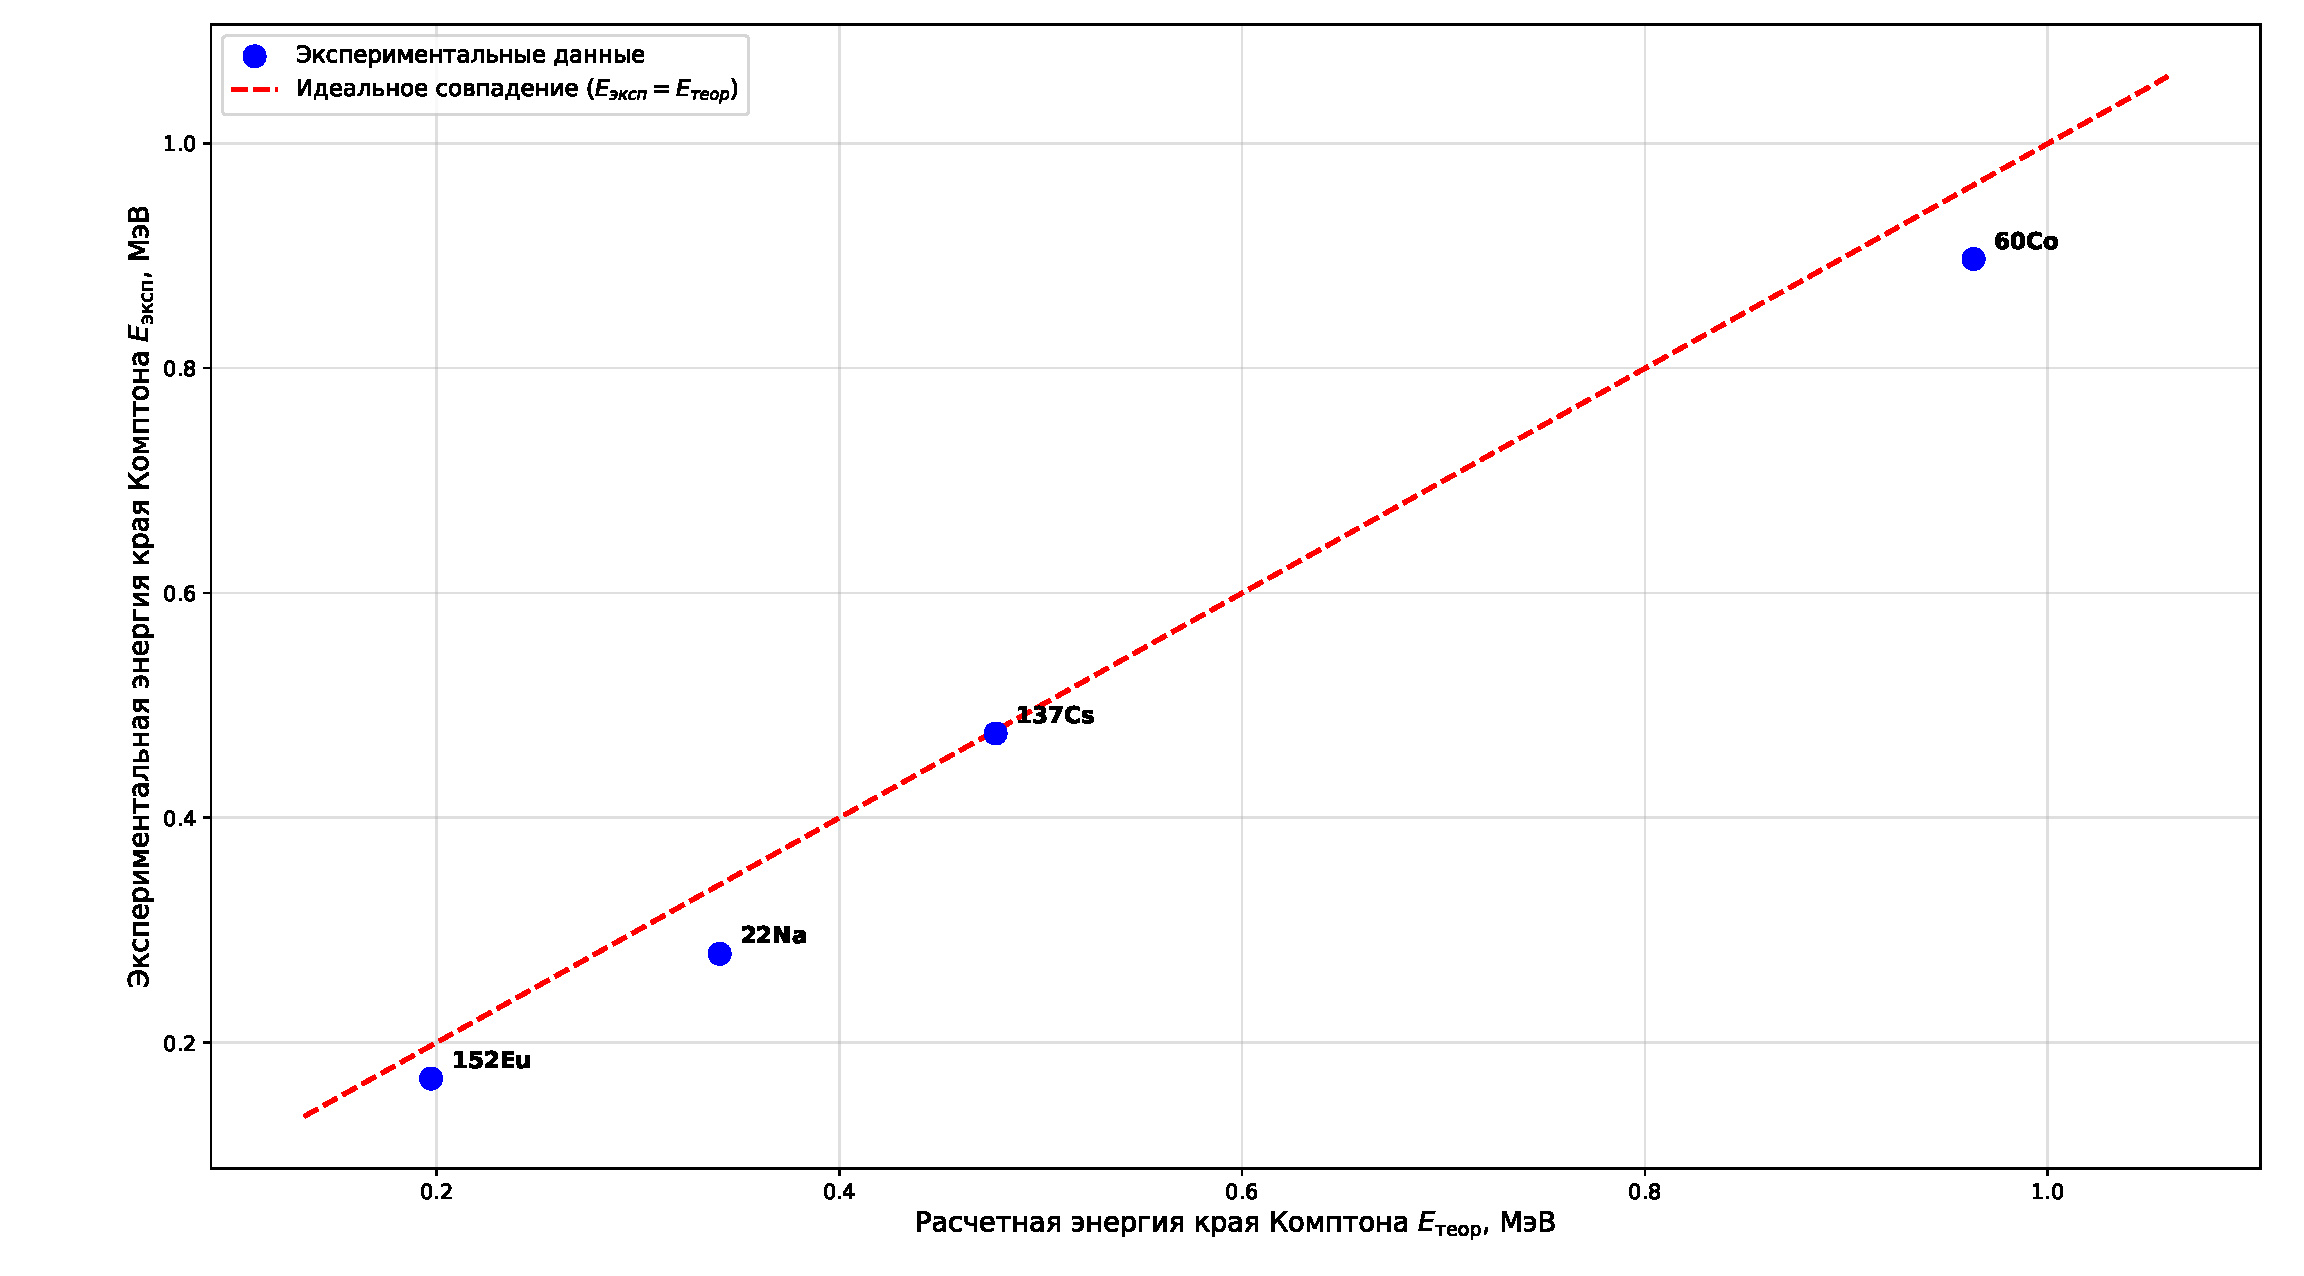
\includegraphics[width=0.7\textwidth]{5.pdf}
    \caption{Зависимость экспериментальной энергии края Комптона от расчетной. Пунктирная прямая соответствует идеальному совпадению $E_{\text{эксп}} = E_{\text{теор}}$.}
    \label{fig:compton_edge}
\end{figure}

Как видно из графика, точка для $^{137}$Cs демонстрирует практически идеальное совпадение с теорией. Для остальных источников экспериментальные значения лежат несколько ниже теоретических. Это типично для сцинтилляционных спектрометров NaI(Tl) и объясняется двумя факторами:
\begin{enumerate}
    \item Конечным энергетическим разрешением детектора, из-за которого резкий теоретический ``обрыв'' края Комптона размывается в пологий спад, и его визуальное определение смещается в сторону меньших энергий.
    \item Наложением экспоненциального фона и пиков обратного рассеяния, что затрудняет точную фиксацию координаты края.
\end{enumerate}
Несмотря на это, общая линейная тенденция сохраняется, что подтверждает правильность идентификации комптоновских краев в спектрах.



\subsubsection*{3. Проверка зависимости $R_i^2 = f(1/E_i)$}

Согласно формуле (6) из описания, энергетическое разрешение сцинтилляционного спектрометра должно удовлетворять зависимости:
\begin{equation}
    R_i = \frac{\text{const}}{\sqrt{E_i}} \quad \implies \quad R_i^2 = \frac{\text{const}^2}{E_i} = k \cdot \frac{1}{E_i}.
\end{equation}
Таким образом, график зависимости $R_i^2$ от $1/E_i$ должен быть линейным. Для проверки этой зависимости были использованы данные таблицы 1. Точки с минимальной энергией для $^{241}$Am ($E \approx 0,021$ МэВ и $E \approx 0,058$ МэВ) исключены из анализа из-за большой погрешности определения разрешения на низких энергиях. Результаты расчётов представлены в таблице 4:

\begin{table}[H]
\centering
\caption{Данные для проверки зависимости $R_i^2 = f(1/E_i)$}
\label{tab:R_squared}
\renewcommand{\arraystretch}{1.2}
\begin{tabular}{|c|c|c|c|c|}
\hline
Источник & $E_i$, МэВ & $R_i$ & $1/E_i$, МэВ$^{-1}$ & $R_i^2$ \\
\hline
$^{60}$Co  & 1,173 & 0,054 & 0,853 & 0,00292 \\
$^{60}$Co  & 1,333 & 0,053 & 0,750 & 0,00281 \\
$^{137}$Cs & 0,662 & 0,072 & 1,511 & 0,00518 \\
$^{22}$Na  & 0,511 & 0,086 & 1,957 & 0,00740 \\
$^{22}$Na  & 1,274 & 0,064 & 0,785 & 0,00410 \\
$^{152}$Eu & 0,123 & 0,100 & 8,130 & 0,01000 \\
$^{152}$Eu & 0,342 & 0,088 & 2,924 & 0,00774 \\
$^{152}$Eu & 0,784 & 0,049 & 1,276 & 0,00240 \\
$^{152}$Eu & 0,972 & 0,046 & 1,029 & 0,00212 \\
$^{152}$Eu & 1,417 & 0,054 & 0,706 & 0,00292 \\
\hline
\end{tabular}
\end{table}

По данным таблицы построен график зависимости $R_i^2$ от $1/E_i$ (рис. X).

\begin{figure}[H]
    \centering
    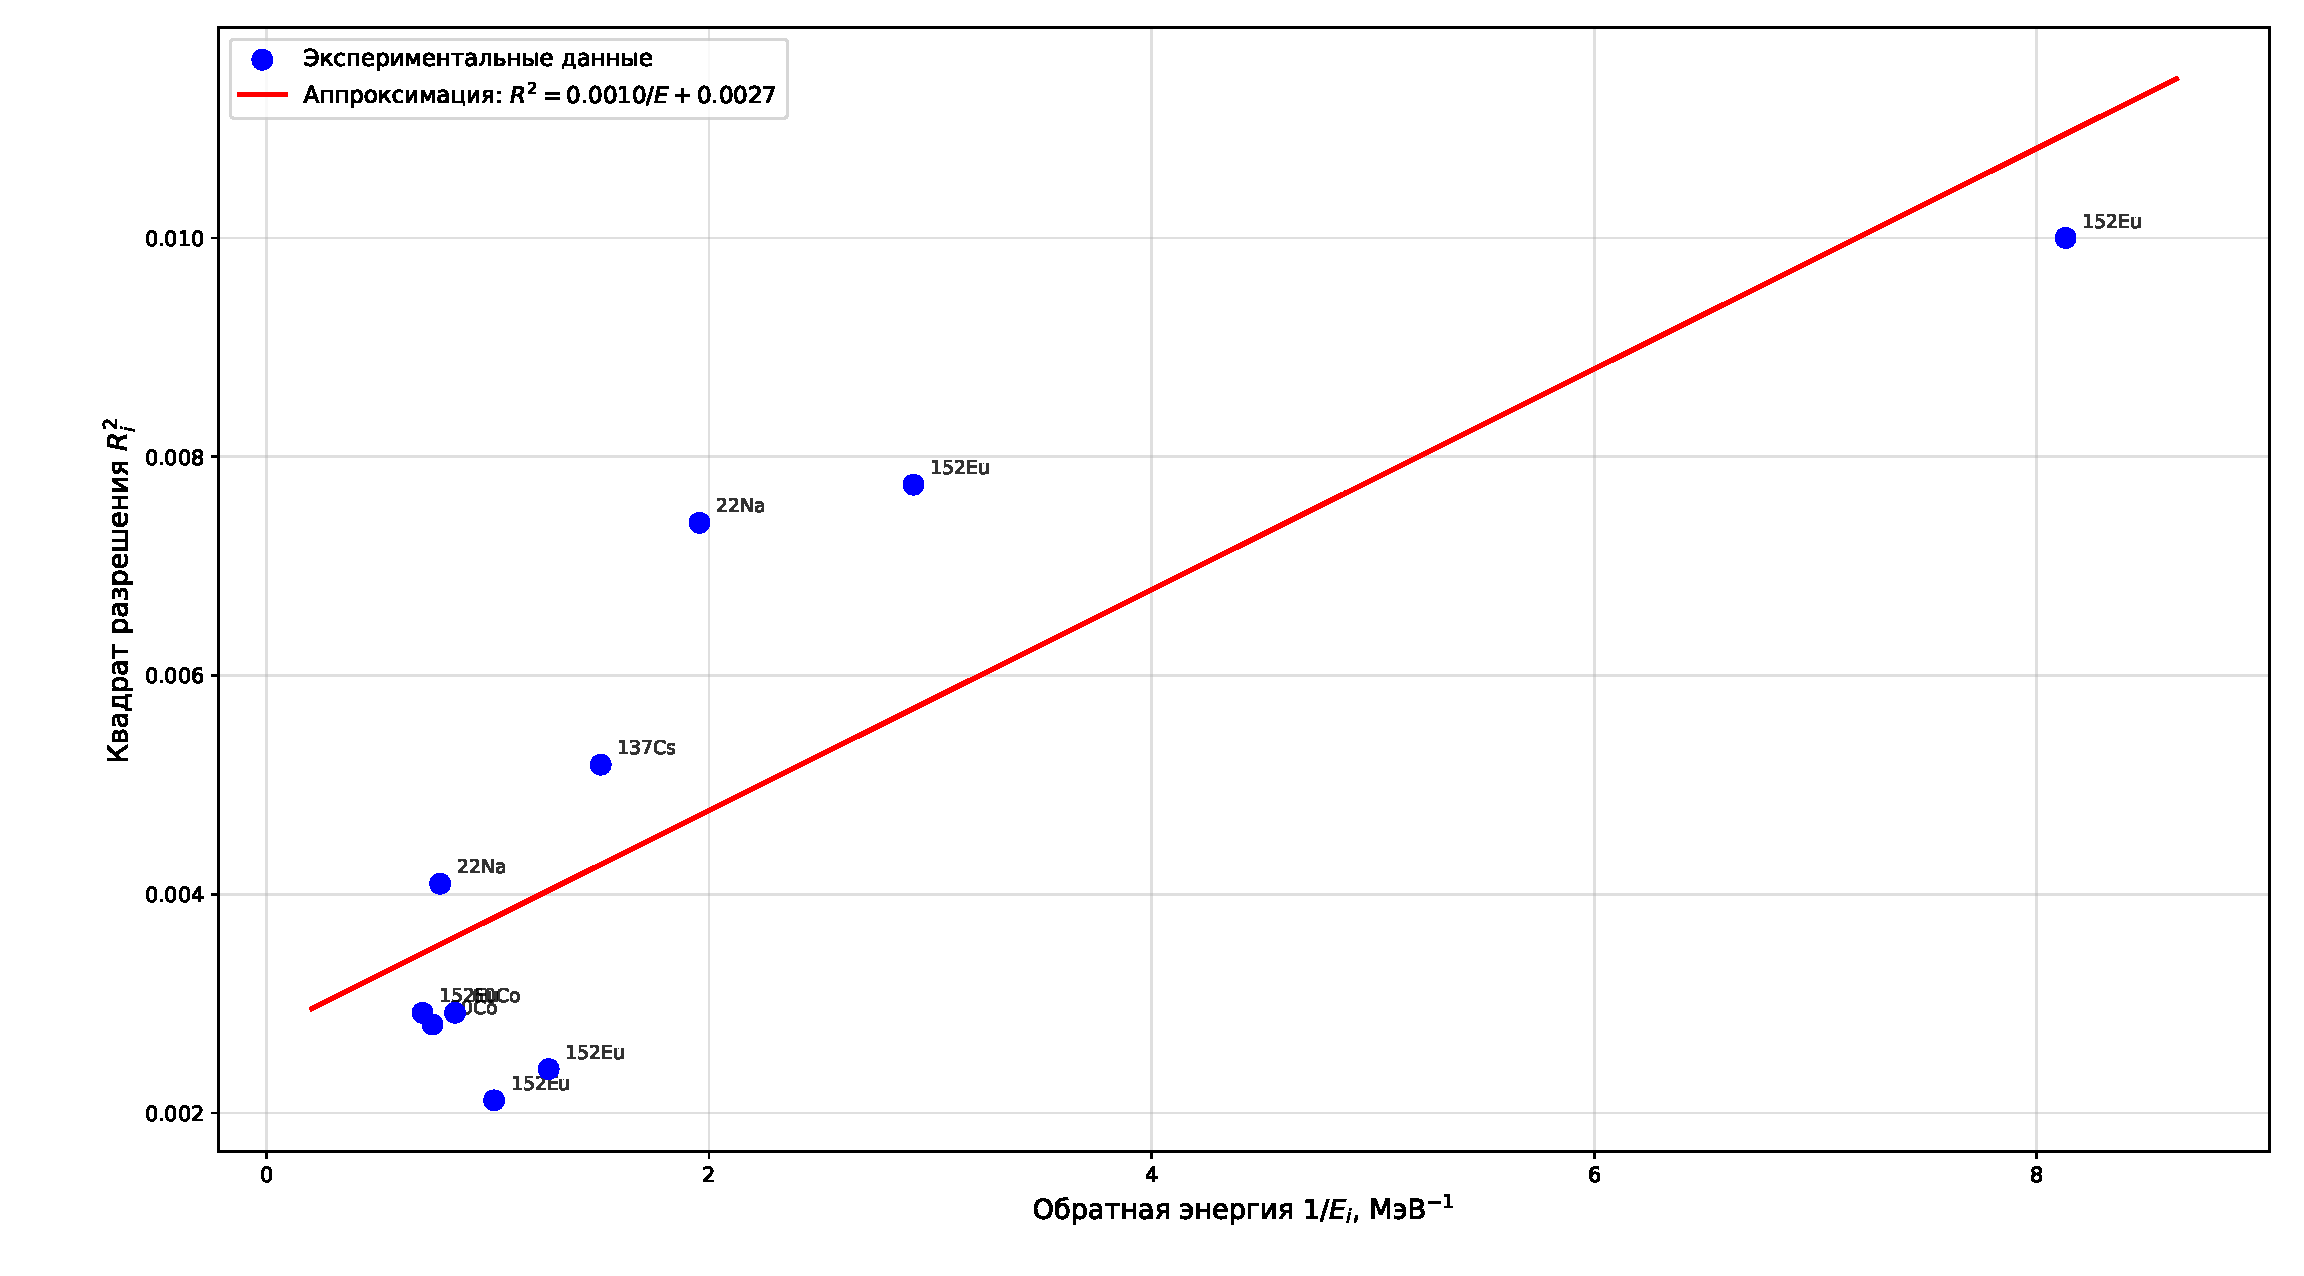
\includegraphics[width=0.9\textwidth]{6.pdf}
    \caption{Зависимость квадрата энергетического разрешения от обратной энергии. Красная прямая --- результат линейной аппроксимации $R^2 = 0,0010/E + 0,0027$.}
    \label{fig:R_squared}
\end{figure}

Как видно из графика, экспериментальные точки в целом следуют линейной тенденции, что качественно подтверждает зависимость $R_i^2 \propto 1/E_i$. Методом наименьших квадратов получена аппроксимация:
\begin{equation}
    R_i^2 = \frac{0,0010}{E_i} + 0,0027.
\end{equation}

Однако разброс точек относительно прямой заметно превышает статистические погрешности. Это объясняется рядом факторов, не учтённых в упрощённой формуле (6):

\begin{enumerate}
    \item \textbf{Вклад шумов электроники и неоднородности светосбора.} Ненулевой свободный член $b = 0,0027$ в аппроксимации соответствует квадратичному вкладу факторов, не зависящих от энергии: $R_{\text{шум}} = \sqrt{0,0027} \approx 5,2\%$. Это типичное значение для спектрометра на основе NaI(Tl). Полная формула разрешения имеет вид $R^2 = k/E + R_{\text{шум}}^2$.
    
    \item \textbf{Нелинейность светового выхода NaI(Tl).} При низких энергиях (ниже $\sim 100$ кэВ) световой выход кристалла перестаёт быть строго пропорциональным энергии, что приводит к дополнительному ухудшению разрешения. Это особенно заметно для точки $^{152}$Eu при $E = 0,123$ МэВ ($1/E \approx 8,1$ МэВ$^{-1}$), которая наиболее сильно отклоняется от прямой.
    
    \item \textbf{Наложение пиков в спектре $^{152}$Eu.} Этот источник имеет очень плотный спектр с большим числом близких $\gamma$-линий. При аппроксимации гауссианом пики могут перекрываться, что искусственно завышает ширину и ухудшает разрешение. Это объясняет отклонения точек $^{152}$Eu при $E = 0,123$ МэВ и $E = 1,103$ МэВ.
    
    \item \textbf{Самопоглощение в источнике.} Для низкоэнергетических $\gamma$-квантов самопоглощение в материале источника искажает форму пика, добавляя асимметрию и увеличивая измеренную ширину на половине высоты.
\end{enumerate}

Несмотря на указанные отклонения, общая линейная зависимость $R_i^2 \sim 1/E_i$ прослеживается, что подтверждает статистическую природу основного вклада в энергетическое разрешение сцинтилляционного спектрометра.



\subsubsection*{4. Оценка параметров импульса ФЭУ}

Форма импульсов на выходе ФЭУ описывается выражением:
\begin{equation}
    U(t) = \text{const} \cdot e^{-t/RC} \left(1 - e^{-t/\tau_0}\right),
\end{equation}
где $\tau_0$ --- время высвечивания сцинтиллятора, $RC$ --- постоянная времени анодной цепи.

По осциллограмме были оценены характерные времена импульса:
\begin{itemize}
    \item \textbf{Время нарастания} (передний фронт) $\sim 1$ мкс. Поскольку передний фронт определяется временем высвечивания $\tau_0$, оцениваем $\tau_0 \approx 0,5$ мкс/%(с учётом того, что время нарастания от 10\% до 90\% амплитуды составляет $\approx 2{,}2\,\tau_0$).
    \item \textbf{Время спада} до уровня $1/e$ от максимума (задний фронт) $\sim 5$ мкс. Это время непосредственно соответствует постоянной времени $RC$, следовательно, $RC \approx 5$ мкс.
\end{itemize}

Проверим условие применимости формулы (7): $RC \gg \tau_0$. В нашем случае:
\begin{equation}
    \frac{RC}{\tau_0} \approx \frac{5 \text{ мкс}}{0{,}5 \text{ мкс}} = 10.
\end{equation}
Условие $RC \gg \tau_0$ выполняется, причём соотношение $RC \approx 10\,\tau_0$ попадает в рекомендуемый диапазон $RC = (5 \div 10)\tau_0$, указанный в методичке.

Полученное значение $\tau_0 \approx 0{,}5$ мкс имеет правильный порядок величины для сцинтиллятора NaI(Tl) (табличное значение $\tau_0 \approx 0{,}23$ мкс).% Небольшое завышение экспериментальной оценки объясняется конечной полосой пропускания осциллографа и влиянием электронной схемы на форму переднего фронта импульса.


\subsubsection*{5. Зависимость энергии пика обратного рассеяния от энергии фотопика}

Согласно формуле (2) из методички, энергия пика обратного рассеяния $E_{\text{обр}}$ жестко связана с энергией первичного фотопика $E_\gamma$ кинематикой комптоновского рассеяния на угол $180^\circ$:
\begin{equation}
    E_{\text{обр}} = \frac{E_\gamma}{1 + 2E_\gamma / m_e c^2},
\end{equation}
где $m_e c^2 = 0,511$ МэВ --- энергия покоя электрона.

Для проверки этой зависимости мы использовали экспериментальные значения энергий пиков обратного рассеяния, полученные ранее из калибровочной зависимости, и сопоставили их с теоретическими расчетами для соответствующих фотопиков. Результаты сведены в таблицу 4.

\begin{table}[H]
\centering
\caption{Сравнение экспериментальных и расчетных энергий пика обратного рассеяния}
\label{tab:backscatter}
\renewcommand{\arraystretch}{1.2}
\begin{tabular}{|c|c|c|c|}
\hline
Источник & $E_\gamma$, МэВ & $E_{\text{обр}}^{\text{эксп}}$, МэВ & $E_{\text{обр}}^{\text{теор}}$, МэВ \\
\hline
$^{22}$Na  & 0,511 & 0,178 & 0,170 \\
$^{137}$Cs & 0,662 & 0,198 & 0,184 \\
$^{60}$Co  & 1,173 & 0,229 & 0,210 \\
\hline
\end{tabular}
\end{table}

По данным таблицы построен график зависимости $E_{\text{обр}}$ от $E_\gamma$ (рис. X).

\begin{figure}[H]
    \centering
    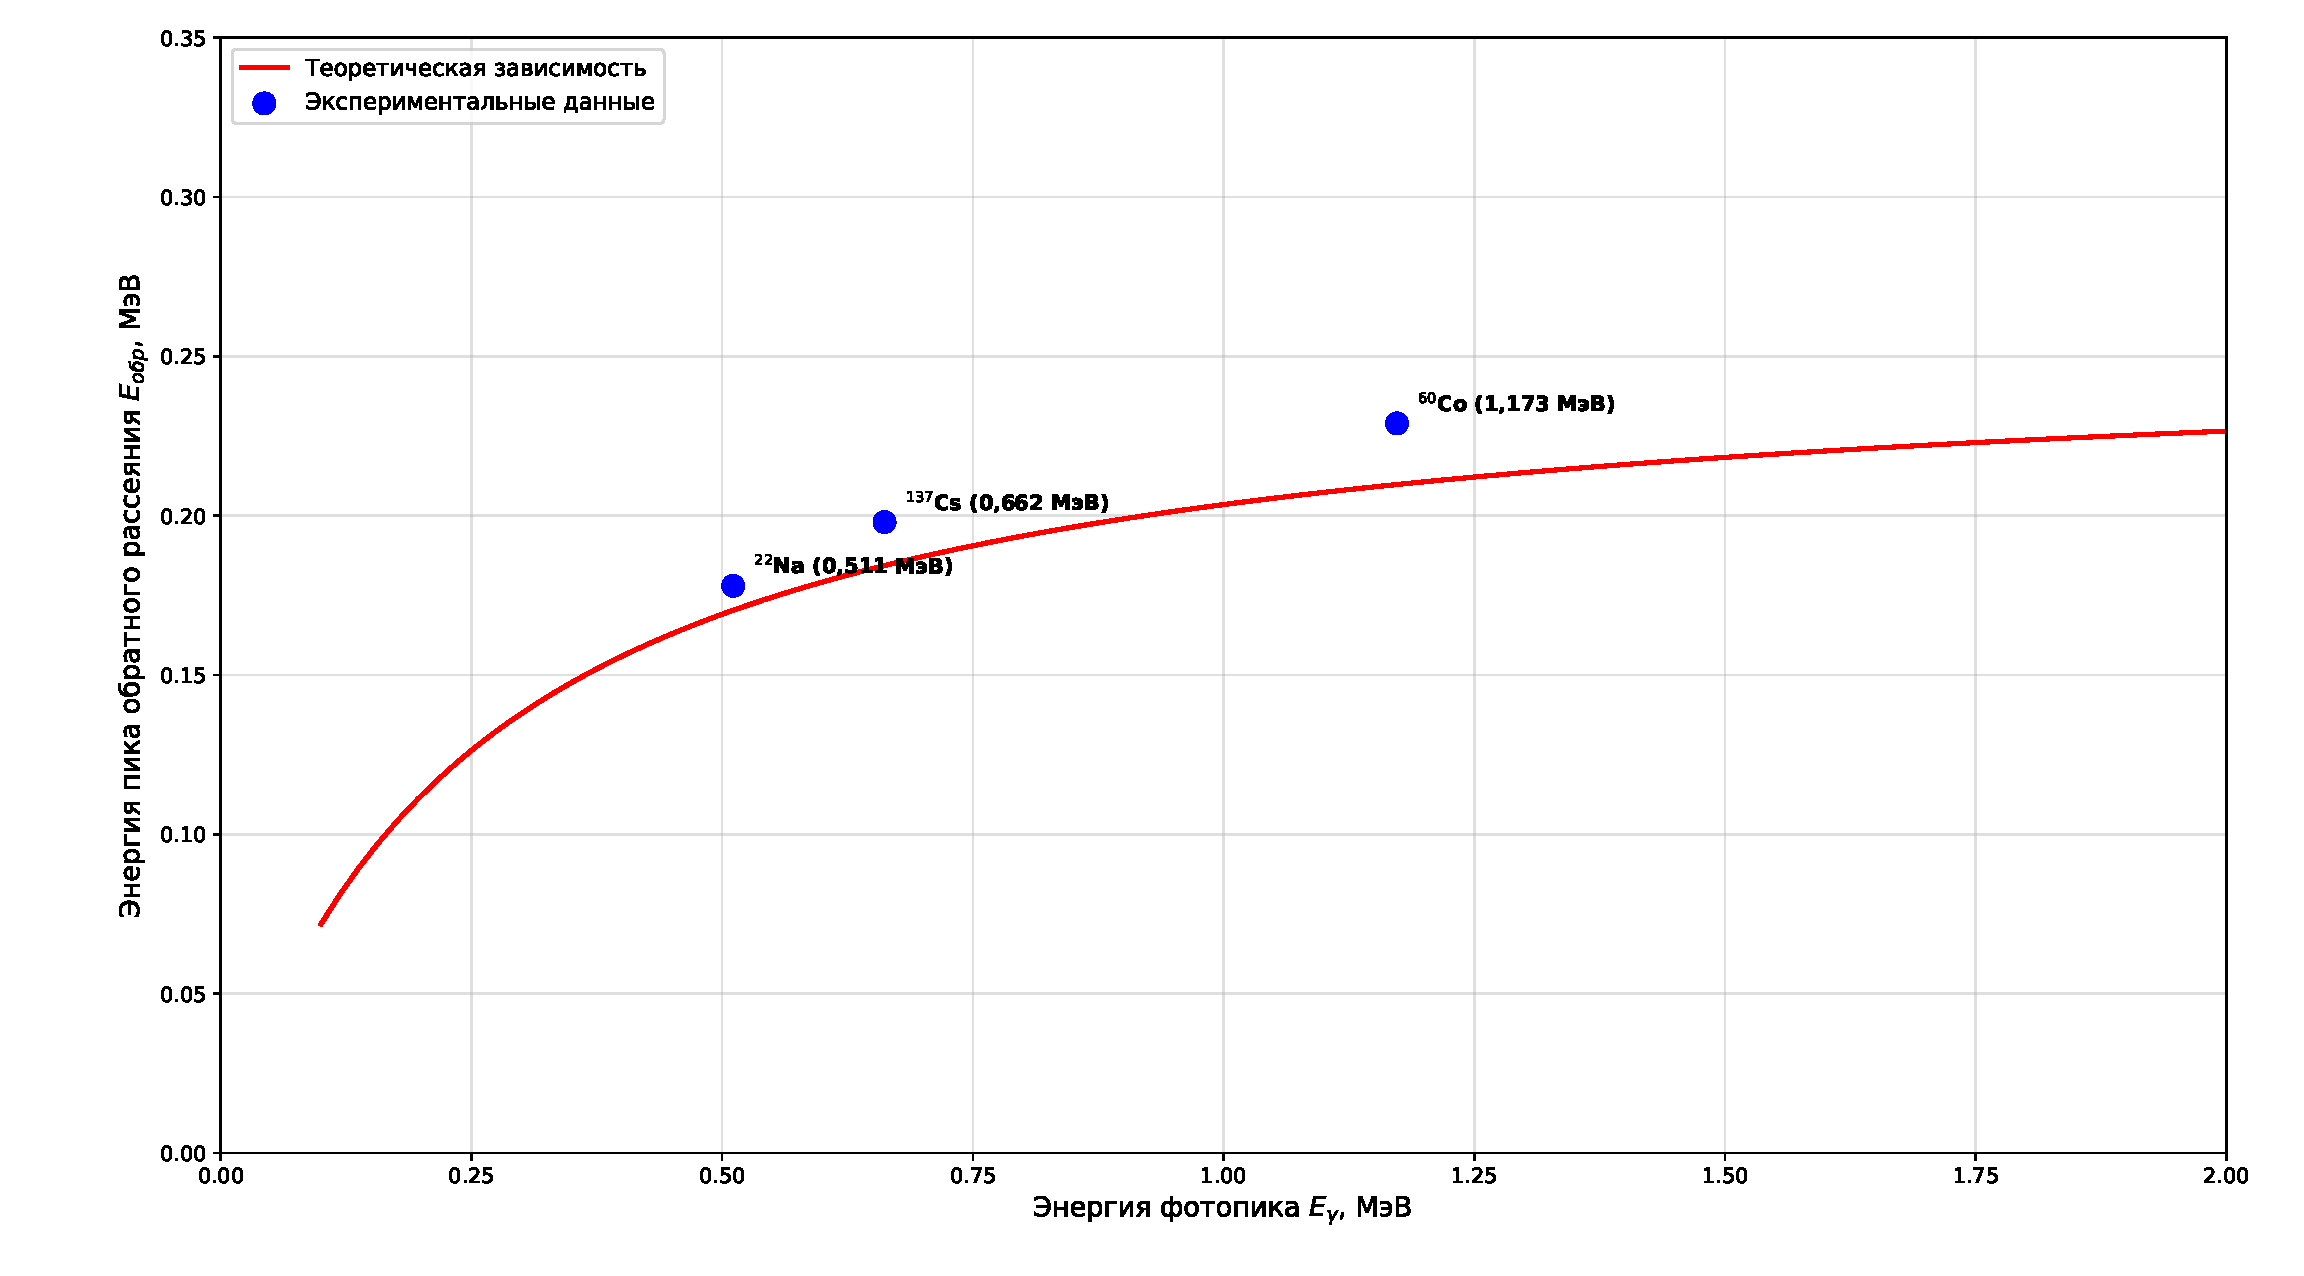
\includegraphics[width=0.8\textwidth]{7.pdf}
    \caption{Зависимость энергии пика обратного рассеяния от энергии фотопика. Сплошная линия --- теоретическая кривая, точки --- экспериментальные данные.}
    \label{fig:backscatter}
\end{figure}

Как видно из графика и таблицы, экспериментальные точки качественно ложатся на теоретическую кривую. Небольшие систематические завышения экспериментальных значений ($E_{\text{обр}}^{\text{эксп}} > E_{\text{обр}}^{\text{теор}}$) на $\sim 0,01$--$0,02$ МэВ являются типичными для сцинтилляционных спектрометров NaI(Tl). Это объясняется конечным энергетическим разрешением детектора, из-за которого комптоновское плато и пик обратного рассеяния «размываются» и сливаются, а также возможным частичным поглощением рассеянных фотонов в материалах самой установки, что смещает максимум аппроксимирующего гауссиана в сторону больших энергий.

Тем не менее, общая нелинейная зависимость с насыщением при высоких энергиях ($E_{\text{обр}} \to m_e c^2 / 2 \approx 0,255$ МэВ при $E_\gamma \to \infty$) четко прослеживается, что подтверждает комптоновскую природу данного пика.


\subsubsection*{6. Энергия характеристического излучения свинца}

Характеристическое рентгеновское излучение свинца возникает при выбивании электронов с внутренних оболочек атомов свинца (из которого изготовлена защита детектора) под действием гамма-квантов. При переходе электронов с внешних оболочек на освободившиеся вакансии испускаются кванты характеристического излучения.

Для свинца ($Z=82$) наиболее интенсивными являются линии $K$-серии:
\begin{itemize}
    \item $K_\alpha$-линия: $E_{\text{теор}} \approx 73\text{--}75$ кэВ ($0,073\text{--}0,075$ МэВ);
    \item $K_\beta$-линия: $E_{\text{теор}} \approx 85$ кэВ ($0,085$ МэВ).
\end{itemize}

Из экспериментальных данных (таблица 1) положения пиков, идентифицированных как излучение свинца для разных источников, находятся в следующем диапазоне:
\begin{itemize}
    \item $^{60}$Co: $E_{\text{эксп}} \approx 0,073$ МэВ
    \item $^{137}$Cs: $E_{\text{эксп}} \approx 0,074$ МэВ
    \item $^{22}$Na: $E_{\text{эксп}} \approx 0,076$ МэВ
    \item $^{152}$Eu: $E_{\text{эксп}} \approx 0,084$ МэВ
\end{itemize}

Среднее экспериментальное значение энергии составляет $E_{\text{эксп.ср}} \approx 0,077$ МэВ ($77$ кэВ). 

Полученные экспериментальные значения отлично согласуются с табличными энергиями $K$-серии характеристического излучения свинца. Небольшой разброс значений (от $0,073$ до $0,084$ МэВ) и наличие пика при $0,084$ МэВ объясняются наложением $K_\alpha$ и $K_\beta$ линий, которые из-за конечного энергетического разрешения детектора NaI(Tl) на низких энергиях не всегда разрешаются в виде двух отдельных пиков, а регистрируются как единый уширенный пик или пик со смещённым центром тяжести.

\section*{Вывод}

В ходе выполнения работы был исследован принцип действия и основные характеристики сцинтилляционного $\gamma$-спектрометра на основе кристалла NaI(Tl). 

Основные полученные результаты:
\begin{enumerate}
    \item \textbf{Калибровка:} Проведена энергетическая калибровка спектрометра по известным источникам ($^{60}$Co, $^{137}$Cs, $^{22}$Na). Получена линейная зависимость $N = (1336,6 \pm 6,1) \cdot E + (65,4 \pm 6,4)$ с высоким коэффициентом детерминации ($R^2 \approx 0,999$), что подтверждает линейность отклика установки.
    \item \textbf{Идентификация спектров:} С использованием калибровки определены энергии фотопиков источников $^{241}$Am и $^{152}$Eu. Также зарегистрировано и идентифицировано характеристическое рентгеновское излучение свинцовой защиты ($E \approx 73\text{--}85$ кэВ).
    \item \textbf{Комптоновское рассеяние:} Экспериментальные значения энергий края Комптона и пика обратного рассеяния хорошо согласуются с теоретическими расчетами по формулам кинематики комптоновского рассеяния.
    \item \textbf{Энергетическое разрешение:} Подтверждена теоретическая зависимость квадрата разрешения от обратной энергии ($R^2 \propto 1/E$). Анализ аппроксимации позволил оценить постоянный вклад шумов электроники и неоднородности светосбора ($R_{\text{шум}} \approx 5\%$), что типично для NaI(Tl).
    \item \textbf{Параметры импульса:} По осциллограммам оценены временные характеристики импульса ФЭУ: время высвечивания сцинтиллятора $\tau_0 \approx 0,5$ мкс и постоянная времени анодной цепи $RC \approx 5$ мкс. Полученное соотношение $RC \approx 10\tau_0$ удовлетворяет условию $RC \gg \tau_0$, необходимому для корректной формы импульса.
\end{enumerate}

Таким образом, поставленные задачи выполнены, а полученные экспериментальные данные подтверждают теоретические модели взаимодействия $\gamma$-излучения с веществом и принципы работы сцинтилляционного детектора.



\end{document}